\documentclass[mathserif]{beamer}
\usetheme{Luebeck}
%\usepackage[francais]{babel}
\usepackage[utf8]{inputenc} % Uses the utf8 input encoding
\usepackage[T1]{fontenc} % Use 8-bit encoding that has 256 glyphs

\usepackage[nomath]{kpfonts}
\usepackage{eulervm}
%\usepackage{default}

\usepackage{amsthm}
\usepackage{amssymb}
\usepackage{xparse}
\usepackage{thmtools}
\usepackage{stackrel}

%shortcuts
\newcommand{\R}{\mathbb{R}}
\newcommand{\C}{\mathbb{C}}
\newcommand{\Z}{\mathbb{Z}}
\newcommand{\N}{\mathbb{N}}
\newcommand{\fii}{\varphi}
\newcommand{\dd}{\mathrm{d}}
\newcommand{\CP}{\mathbb{CP}}
\renewcommand{\S}{\mathbb{S}}
\DeclareMathOperator{\Sp}{Sp}
\DeclareMathOperator{\tr}{tr}
\DeclareMathOperator{\dist}{dist}

% theorems configuration

\makeatletter
\newtheoremstyle{indented}
{7pt} %vertical space before
{7pt} % vertical space after
{} %{\addtolength{\@totalleftmargin}{2.5em}
	%\addtolength{\linewidth}{-3.5em}
	%\parshape 1 3.5em \linewidth} %body font
{1.5em} %indent
{\bfseries} %header font
{.} %punctuation
{.5em} %horizontal space after header
{} %header specification

\theoremstyle{definition}

\newtheorem{defn}{Définition}[section]

\theoremstyle{plain}
%\newtheorem*{theorem*}{Theorem}

\newtheorem{thm}{Théorème}

\renewcommand{\thetheorem}{\Alph{theorem}}
\newenvironment{preuve}{
	\noindent \textbf{Proof. }}{\hfill $\square$\medskip\par}

\newtheorem{exemple}[defn]{Example}
\newtheorem{prop}[defn]{Proposition}
\newtheorem{corr}[defn]{Corollary}
\newtheorem{por}[defn]{Porisme}
\newtheorem{ex}[defn]{Example}
\newtheorem{lem}[defn]{Lemma}
\newtheorem{conj}{Conjecture}
\newtheorem{ax}{Axiom}  %Axioms have their own numerotation

\theoremstyle{definition}
\newtheorem{rem}[defn]{Remark} %remarks are not indented
\newtheorem{rems}[defn]{Remarks}

%--------------
% Mise en page mathématique
%--------------
\addtolength{\jot}{.2em}


\title[Low-energy spectrum of Toeplitz Operators]{Low-energy spectrum of Toeplitz Operators}
\author[Alix Deleporte]{Alix Deleporte\\Advisor : Nalini Anantharaman}
\institute[IRMA]{Institut de Recherche Mathématique
  Avancée\\Université de Strasbourg}

\AtBeginSection
{
	\begin{frame}
		\frametitle{Plan}
		\tableofcontents[currentsection]
	\end{frame}
	
}

\newcommand{\spline}{\hline}
\renewcommand{\arraystretch}{1.3}
\begin{document}
\begin{frame}
	\titlepage
\end{frame}

\section{Toeplitz opreators}
\subsection{Toeplitz operators on $\C^n$}
\begin{frame}
  \frametitle{Bargmann spaces}
  \begin{itemize}
  \item Original idea: express Quantum Mechanics directly in phase
    space.
  \uncover<2->{\item The standard $L^2(\R^n)$ is replaced with the \emph{Bargmann
      space}, with parameter $N>0$:
$$B_N=L^2(\C^n)\cap\left\{e^{-\frac N2 |\cdot|^2}f,\,f\text{ is
  holomorphic on $\C^n$}\right\}.$$}\vspace{-2em}
  \uncover<3>{\item This is a closed subspace of $L^2(\C^n)$, with reproducing
    kernel
$$\Pi_N(x,y)=\left(\frac N{\pi}\right)^n\exp\left(-\cfrac N2
  |x-y|^2+iN\Im(x\cdot \overline{y})\right).$$}
  \end{itemize}
\vspace{-1em}
\small{[1] Bargmann, V. Comm. Pure Appl. Math. 14, no. 3 (1961): 187–214.}

\end{frame}

\begin{frame}
  \frametitle{Szeg\H{o} kernel}
  Hilbert basis indexed by $\N^{n}$.

$$e_{\nu}=\cfrac{N^{|\nu|}}{\nu_1!\nu_2!\ldots\nu_n!}z^{\nu}e^{-\frac{N|z|^2}{2}}.$$

\uncover<2>{From there one recovers $\Pi_N$ with
$$\Pi_N(x,y)=\sum_{\nu\in \N^n} e_{\nu}(x)\overline{e_{\nu}}(y).$$

The Szeg\H{o} kernel decays exponentially fast away from the diagonal.
}
\end{frame}

\begin{frame}
  \frametitle{Toeplitz quantization}
  Let $f\in C^{\infty}(\C^n,\C)$ bounded. The Toeplitz operator associated
  with $f$ is the bounded operator
\begin{center}
\begin{array}{rcl}
 		T_N(f):B_N(\C^n)&\mapsto & B_N(\C^n)\\
		u& \mapsto& \uncover<2->{\Pi_N(}fu\uncover<2->{)}.
 		\end{array}
\end{center}

\uncover<3->{If $f$ has polynomial growth then $T_N(f)$ is an unbounded operator
with dense domain.}
\uncover<4>{\begin{itemize}
\item If $f$ is real-valued then $T_N(f)$ is ess. self-adjoint.
\item If moreover $f\geq 0$ then $T_N(f)\geq 0$.

\end{itemize}}
\end{frame}

\begin{frame}
  \frametitle{Composition of Toeplitz operators}
  \begin{itemize}
  \item If $f$ is holomorphic then $T_N(f)=f$.
  \item If $f$ is anti-holomorphic then $T_N(f)=f(N^{-1}\partial+\frac z2).$

\uncover<2->{\item The Toepliz quantization is \emph{anti-Wick}: if $f$ is
  anti-holomorphic and $h$ is holomorphic then
$$T_N(fgh)=T_N(f)T_N(g)T_N(h).$$}
\uncover<3>{\item More generally, composition yields a formal series:
$$T_N(f)T_N(g)=T_N\left(fg+N^{-1}C_1(f,g)+N^{-2}C_2(f,g)+\cdots)$$

$C_j$ is a bidifferential operator of total order $2j$.}
\end{itemize}
\end{frame}



\subsection{Toeplitz operators on compact manifolds}
\begin{frame}
  \frametitle{Hardy spaces and Szeg\H{o} kernel}
  \begin{itemize}
  \item Geometrical setting: compact K\"ahler manifold $M$.\\
    \begin{minipage}{0.37\linewidth}\begin{itemize}
    \item Symplectic form
    \item Complex structure
    \end{itemize}
\end{minipage}
\uncover<2->{\begin{minipage}{0.52\linewidth}

$\biggl\}$ Compatibility condition
\end{minipage}}
\uncover<3->{\item Complex line bundle $L\to M$ with curvature $-i\omega$.}
\uncover<4->{\item Hardy space $H_N(M,L)$ of holomorphic sections of $L^{\otimes N}$.}
\uncover<5->{\item Szeg\H{o} projector $S_N:L^2(M,L^{\otimes N})\to H_N(M,L).$}
  \end{itemize}
\uncover<6>{The spaces $H_N(M,L)$ are finite-dimensional in that case. The
line bundles $L^{\otimes N}$ correspond to the weights $e^{-\frac N2
  |\cdot|^2}$ in the flat case.}
\vspace{1em}

\small{[2] Woodhouse, N. Geometric Quantization. Oxford University Press, 1997.}
\end{frame}

\begin{frame}
  \frametitle{Algebra of Toeplitz operators}
  \begin{itemize}
  \item The Szeg\H{o} kernel $S_N$ has a full expansion near the
    diagonal, and decays far from it.
  \uncover<2->{\item Indeed $S_N$ can be seen as the $N$-th Fourier mode of a
    Fourier Integral Operator with the diagonal as critical set.}
\uncover<3->{\item The dominant term is always $\Pi_N$.}
  \uncover<4>{\item Toeplitz operators form a $C^{*}$-algebra as previously.} 
  \end{itemize}
\vspace{2em}

\small{[3] Boutet de Monvel, L, Sjöstrand, J. Journées EDP 34–35 (1975): 123–64.

[4] Charles, L. Comm. Math. Phys. 239, no. 1–2 (2003): 1–28.

[5] Berman, R., Berndtsson, B., Sjöstrand, J.,  Arkiv För Matematik
46, no. 2 (2008).

[6] Kordyukov, Y. ArXiv Preprint ArXiv:1703.04107, 2017.
}

 

\end{frame}

\begin{frame}
  \frametitle{An example: the 2D sphere}
  Here $M=\mathbb{S}^2$. In the stereographic projection, $L$
  corresponds to the weight $z\mapsto \frac{1}{1+|z|^2},$ so
  that \begin{align*}H_N(M,L)&\simeq \left\{f\text{ holomorphic in
                               $\C$},\,\int_{\C}\cfrac{|f|^2}{(1+|z|^2)^{N+2}}<\infty\right\}\\
                             &=\C_N[X].\end{align*}
\uncover<2>{In the canonical basis $\binom{N}{k}^{-\frac 12}X^k$, the Toeplitz
quantization of the three base coordinates on $\mathbb{S}^2$ are the Spin
matrices with spin $S=\frac {N-1}2$.}
\end{frame}


\section{Spin systems in the semiclassical limit}
\begin{frame}
  \frametitle{General spin systems}
\begin{itemize}
  \item Systems with $n$ spins correspond to the K\"ahler manifold
  $(\mathbb{S}^2)^n$.

\item We are interested in \emph{antiferromagnetic} systems. Let $G=(V,E)$
  a finite graph, the antiferromagnetic symbol on
  $(\mathbb{S}^2)^{|V|}$ is set to $$h_{AF}=\sum_{(i,j)\in
    E}x_ix_j+y_iy_j+z_iz_j.$$
\uncover<2>{\item If the graph is bipartite, then the minimum is reached when two
  neighbours always have opposite values.}
\end{itemize}
\end{frame}

\begin{frame}
  \frametitle{Frustrated systems}
  \begin{itemize}
  \item In frustrated systems, the previous solution is not possible.
  \uncover<2->{\item If the graph is ``made with triangles'', then on each triangle
    the sum of the vectors should be zero.}
  \uncover<3>{\item This yields a \emph{degenerate} minimal set, which is not a
    manifold.
  \item What behaviour should one expect for the eigenvectors with
    minimal eigenvalue
    of $T_N(h_{AF})$?}
  \end{itemize}
\vspace{1em}

\small{[7] Douçot, B., and Simon, P.,  J. Physics A: Math and General 31, no. 28 (1998)}

\end{frame}

\section{Melin estimate and localization}
\subsection{General result}
\begin{frame}
  \frametitle{Characteristic value}
  Can one improve the lower bound $f\geq 0\Rightarrow T_N(f)\geq 0$ ?
  \begin{itemize}
  \item If $q$ is a quadratic form in $\C^n$, the minimal eigenvalue
    of $T_N(q)$ is $N^{-1}\mu(q)$ with $$\mu(q)=N^{-1}(Tr^+(q)+\frac
    12 \tr(q)).$$
  \uncover<2>{\item Here, up to a
    symplectomorphism, $$q=\sum_{i=1}^{r}\lambda_i(q_i^2+p_i^2)+\sum_{i=r+1}^{r+r'}p_i^2,$$
    so $$Tr^+(q)=\sum_{i=1}^r\lambda_i.$$
}

\end{itemize}
\end{frame}

\begin{frame}
\frametitle{Melin estimate}
\begin{itemize}
  \item Local result: for sections $u$ sufficiently concentrated around a
    minimal point of $f$ where the Hessian matrix is $q$, one has $\langle
    u,T_N(f)u\rangle \geq N^{-1}\mu(q)+CN^{-1-\epsilon}$.
  \uncover<2>{\item Global result: if $\mu_{inf}$ is the infimum of $\mu$ over all
    minimal points, then $$T_N(f)\geq N^{-1}\mu_{inf}+N^{-1-\epsilon}.$$}
  \end{itemize}

\small{
[8] Melin, A. Arkiv För Matematik 9, no. 1 (1971): 117–140}

\end{frame}

\begin{frame}
  \frametitle{Ideas for the proof}
  \begin{itemize}
  \item Local result: use the fact that the Szeg\H{o} kernel is
    equivalent to the $\C^n$ case near the diagonal, as $N\to
    +\infty$.
  \uncover<2>{\item Global result: pick a covering of the manifold with small open sets
    corresponding to the section, and ask
    that the section is relatively smaller at the intersection of the
    open sets than elsewhere.}
  \end{itemize}
\end{frame}

\subsection{Localization of the ground state}
\begin{frame}
  \frametitle{A general localization result}
  \begin{thm}
    Let $f\in C^{\infty}(M,\R)$ with $\min(f)=0$.
    Then any sequence $(u_N)$ of normalized ground states of $T_N(f)$ is such that
$$\int_{f(x)\geq N^{-1+\delta}}|u_N(x)|^2 \dd Vol=O(N^{-\infty}).$$
  \end{thm}

  \uncover<2->{Indeed, the first eigenvalue is $O(N^{-1})$, so that $\langle
  u_N,fu_N\rangle=O(N^{-1})$.}

\uncover<3>{By induction, $\langle u_N,f^ku_N\rangle = O(N^{-k})$,
  hence the claim.}
\end{frame}

\begin{frame}
\frametitle{Subprincipal effects on localization}
  \begin{thm}
    Let $f\in C^{\infty}(M,\R)$ with $\min(f)=0$. Let $V$ at positive
    distance from $\{\mu=\mu_{min}\}$.
    Then, with $(u_N)$ as previously one has $$\int_{V}|u_N|^2\dd Vol=O(N^{-\infty}).$$
  \end{thm}
\uncover<2>{The proof uses the Melin estimates.}
\end{frame}

\begin{frame}
  \frametitle{Expansions in the regular case}
  The regular case is a generalization of Helffer-Sj\"ostrand's
  ``miniwells''.
If $\mu$ is only minimal at one point $x_0$ near which $\{f=0\}$ is
    an isotropic submanifold, and the minimum is non-degenerate, then
    \begin{itemize}
    \item The first eigenvalue is simple and admits an expansion in
      powers of $N^{-\frac 14}$.
    \item The first eigenvector concentrates at speed $N^{-\frac 12+}$
      on $\{f=0\}$ and at speed $N^{-\frac 14+}$ on $x_0$ along
      $\{f=0\}$.
    \end{itemize}

\vspace{2em}
\small{[9] Helffer, B., Sjöstrand, J. Current Topics in PDEs, 1986, 133–186.}
\end{frame}

\begin{frame}
  \frametitle{Tools for the regular case}
  For the regular case we use quantizations of symplectic maps:

If $\sigma:U\to V$ is a local symplectomorphism between two K\"ahler
manifolds $M$ and $N$, then there is a sequence of maps
$\mathfrak{S}_N:M\to N$, such that, when it acts on sequences of
sections microlocalizing on $U$, 

\begin{itemize}
\item $\mathfrak{S}_N$ is an isometry modulo $O(N^{-\infty})$ error.
\uncover<2->{\item $\mathfrak{S}_NT_N(h)\mathfrak{S}_N^{-1}=T_N(\sigma\circ h + N^{-1}g_1+N^{-2}g_2+\cdots).$}
\end{itemize}

\uncover<3>{At the minimal points, the subprincipal symbol $g_1$ is
  prescribed by the Melin estimates on both sides.}
\end{frame}

\begin{frame}
  \frametitle{A singular toy model}
\begin{itemize}
  \item Consider the following symbol on $\C^n$: $y_1^2+y_2^2+x_1^2x_2^2$.

\item The minimal set is a union of two lines $(x_1,0,0,0)$ and
$(0,x_2,0,0)$. Along the first, $\mu=|x_1|$.

\uncover<2->{\item For this model the concentration speed on $0$ is $N^{-\frac
    13+}$.}
\uncover<3->{\item What is the rate of decay along the minimal set?}
\end{itemize}
\end{frame}

% \begin{frame}\frametitle{Introduction}
% \begin{center}
% 	\begin{tabular}{|c|c|}
% 		\spline
% 	    Classical mechanics & Quantum mechanics\\
% 		\spline
% 		Symplectic manifold $M$ & Hilbert Space $H$\\ 
% 		\spline 
% 		Function $a\in C^{\infty}(M,\R)$ & Self-adjoint
%                                                    operator $A\in L(H)$\\
% 		\spline
%                 Hamiltonien flow of $a$ & Flow of $e^{itA/\hbar}$\\
% 		\spline
% 		Poisson Bracket & Lie Bracket\\
% 		\spline
% 	\end{tabular}\end{center}\vspace{0em}
% 	\begin{itemize}
% 	\uncover<2>{\item Quantization : for a given classical
%           model, how to construct an associated quantum
%           model ?
	
% 	\item Semiclassics : the quantum model is $\hbar$-dependent. What
%           can be said in the $\hbar\to 0$ limit ?}
% 	\end{itemize}
% \end{frame}

% \begin{frame}\frametitle{Introduction}
% 	\begin{itemize}
% 		\item Quantum spins: triplet of self-adjoint matrices
%                   $S_x,S_y,S_z\in M_{2S+1}(\C)$, with $$[S_a,S_b]=\frac{i}{S}\epsilon_{abc}S_c.$$
% 		\item For $S=\frac 12$, one finds the Pauli matrices
% 		$$S_x=\tiny{\frac 12\begin{pmatrix}
% 		0& 1\\1& 0
% 		\end{pmatrix}}\quad S_y=\frac 12\begin{pmatrix}
% 		0& i\\-i& 0
% 		\end{pmatrix}\quad S_z=\frac 12\begin{pmatrix}
% 		1& 0\\0& -1
% 		\end{pmatrix}.$$
% 		\uncover<2>{\item For any finite graph $G$, we wish to study the
%                   following operator acting on $(\C^{2S+1})^{\otimes |G|}$:
% 		$$H=\sum_{e\sim f}S_{x,e}S_{x,f}+S_{y,e}S_{y,f}+S_{z,e}S_{z,f}$$
% 		as $S\to +\infty$.}
% 	\end{itemize}
% \end{frame}

% \section{Toeplitz operators on Bargmann spaces}
% \subsection{Bargmann spaces}
% \begin{frame}\frametitle{Bargmann spaces}
% 	The Bargmann spaces are $L^2$ spaces of holomorphic functions
%         on $\C^n$, with a weight.
% 	\begin{equation*}
% 		B_N(\C^n)=\left\{z\mapsto \exp\left(-\frac N2|z|^2\right)f(z),\,f\text{ holomorphic}\right\}\cap L^2(\C^n)
% 	\end{equation*}
% 	Those are closed subspaces of $L^2(\C^n)$.
% \end{frame}
% \begin{frame}\frametitle{The Szeg\H{o} projector}
% 	Let $\Pi_N$ be the orthogonal projector from $L^2(\C^n)$ onto
%         $B_N(\C^n)$. $\Pi_N$. It admits a Schwartz kernel:
% 	\begin{equation*}
% 		\Pi_N(z,w)=\frac{N^n}{\pi^n}\exp\left[N(-\frac 12 |z-w|^2+i\Im(z\cdot \overline{w}))\right].
% 	\end{equation*}
% 	As $N\to +\infty$, the kernel is exponentially decreasing far
%         from the diagonal. The typical interaction scale is $N^{-1/2}$.
% \end{frame}
% \subsection{Definition}
% \begin{frame}
% \frametitle{Toeplitz operators}
% \begin{defn}
% 	Let $h\in C^{\infty}(\C^n)$ a smooth bounded function, and
%         $N\in \N$. We denote by $T_N(h)$ the Toeplitz operator
%         associated to $h$:
% 	\begin{equation*}
% 		\begin{array}{rcl}
% 		T_N(h):B_N(\C^n)&\mapsto & B_N(\C^n)\\
% 		u& \mapsto& \Pi_N(hu).
% 		\end{array}
% 	\end{equation*}
% \end{defn}
% If $h$ is not bounded, we can construct $T_N(h)$ as an unbounded
% operator on $B_N(\C^n)$. 

% The mapping $h\mapsto T_N(h)$ is linear and adjoint-preserving. If $h$
% is real-valued, then $T_N(h)$ is formally self-adjoint.
% \end{frame}

% \begin{frame}\frametitle{Anti-Wick quantization}
% 		\begin{itemize}
% 		\item<1-> There holds $T_N(1)=1$, and if $h$ is
%                   holomorphic, then$T_N(h)=h$ ; for instance $T_N(z_i)=z_i$.
		
% 		\item<2-> Moreover $T_N(\overline{z}_i)=N^{-1}\partial_i.$
		
% 		\item<3-> If $h:z\mapsto \overline{z}^{\alpha}z^{\beta}$, then $T_N(h)=N^{-|\alpha|}\partial^{\alpha}z^{\beta}$.
		
% 		\item<4-> If $q$ is a definite quadratic form on 
%                   $\R^{2n}$, then $T_N(q)$ has a compact
%                   resolvent. The first eigenvalue
%                   $\mu_N(q)=N^{-1}\mu_1(q)$ is positive.

%                   \begin{equation*}
%                     \mu_1(q)=\min \Sp(Op^W_1(q)) + \frac 12 \tr(q)
%                   \end{equation*}
% 		\end{itemize}
% \end{frame}

% \subsection{Semiclassical properties}
% \begin{frame}\frametitle{Composition and bracket}
% 	\begin{prop}
% 		Let$a$ and $b$ two smooth bounded functions on
%                 $\C^n$. Then there is a sequence $(c_i)_{i\in \N}$ of
%                 smooth bounded functions on $\C^n$, with $c_0=ab$ so
%                 that, as $N\to +\infty$, there holds:
% 		\begin{equation*}
% 			T_N(a)T_N(b)=T_N(c_0)+N^{-1}T_N(c_1)+N^{-2}T_N(c_2)+\ldots
% 		\end{equation*}
		
% 		\uncover<2>{In particular,
% 		\begin{equation*}
% 			[T_N(a),T_N(b)]=\cfrac{i}{N}T_N(\{a,b\})+O(N^{-2}).
% 		\end{equation*}}
% 	\end{prop}
% \end{frame}

% \section{Generalization to K\"ahler manifolds}
% \begin{frame}
% 	\begin{itemize}
% 		\item We wish to generalize Bargmann spaces to other
%                   complex manifolds.
% 		\item As previously, without a good choice of a
%                   weight, the outcome is trivial.
% 		\item<2> Instead of considering weighted spaces, we
%                   will consider spaces of holomorphic sections.
% 	\end{itemize}
% \end{frame}
% \subsection{Hardy spaces}
% \begin{frame}\frametitle{Notations}
% 	\begin{itemize}
% 		\item $M$ is a compact K\"ahler manifold, with
%                   symplectic form $\omega$.
% 		\item $L$ is a complex line bundle on $M$, endowed
%                   with a hermitian structure $h$, so that the
%                   curvature of the Chern connexion is $\omega$.
% 		\item $N\geq 1$ is an integer.
% 	\end{itemize}
% 	\uncover<2->{Then if $s$ is a (continuous) section of
%           $L^{\otimes N}$, one can compute $$\|s\|_{L^2}:=\int_M h_N(s(m))\cfrac{\omega^{\wedge n}}{n!}.$$
% 	By completion, one defines the Hilbert space of square-integrable sections of $L^{\otimes N}$.}
% \end{frame}

% \begin{frame}\frametitle{Hardy spaces}
% 	\begin{defn}
% 		The \emph{N-equivariant Hardy space} is the space
%                 $H_N(M,L)$ of $L^2$ and holomorphic sections of $L^{\otimes N}$.
% 	\end{defn}
% 	This space is finite-dimensional, the dimension is polynomial
%         in $N$ (Riemann-Roch).
% 	\uncover<2>{\begin{defn}
% 		The \emph{Szeg\H{o} projector} $S_N$ is
%                 the orthogonal projector from $L^2(M,L^{\otimes N})$ onto $H_N(M,L)$.
% 	\end{defn}
% 	It always admits a Schwartz kernel ( as a section of
%         $L^{\otimes N}\boxtimes L^{\otimes -N}$) because $H_N(M,L)$ is finite-dimensional.}\end{frame}

% \begin{frame}\frametitle{Toeplitz operators}
% 	\begin{defn}
% 		Let $h\in C^{\infty}(M)$ a smooth function, and $N\in
%                 \N$. We denote by $T_N(h)$ the Toeplitz operator
%                 associated with $h$:
% 		\begin{equation*}
% 		\begin{array}{rcl}
% 		T_N(h):H_N(M,L)&\mapsto & H_N(M,L)\\
% 		u& \mapsto& S_N(hu).
% 		\end{array}
% 		\end{equation*}
% 	\end{defn}
% 	$T_N(h)$ acts on a finite-dimensional space, and it is
%         symmetric when $h$ is real-valued.

% \uncover<2>{Observe that, for any $u,v\in H_N(M,L)$, there
%   holds $$\langle u, T_N(h)v\rangle = \langle u,hv\rangle.$$}
% \end{frame}
% \subsection{Semiclassical properties}
% \begin{frame}\frametitle{Asymptotics for the Szeg\H{o} projector}
% 	\begin{prop}[Boutet-Sjostrand 74]
% 		For every $\epsilon>0$ and $k\in \N$ there exists $C$
%                 such that, for every $N\in \N$:
% 		\begin{equation*}
% 			d(x,y)>\epsilon \Rightarrow |S_N(x,y)|\leq C N^{-k}
% 		\end{equation*}
% 	\end{prop}
% 	\uncover<2>{\begin{prop}[Charles 00, Zelditch 02, Ma 06]
% 		In a convenient system of local coordinates, near any
%                 point of the diagonal, there holds:
% 		\begin{equation*}
% 			S_N(z,w)\simeq\Pi_N(z,w)\left[1+\sum_{k=1}^KN^{-k/2}b_k(\sqrt{N}z,\sqrt{N}w)\right]
% 		\end{equation*}
% 	\end{prop}}
% \end{frame}

% \begin{frame}\frametitle{Composition and bracket}
% 	\begin{prop}[Charles 00, Schlichenmaier 02]
%           Let $a$ and $b$ two smooth functions on $M$. Then
%           there is a sequence $(c_i)_{i\in \N}$ of smooth functions on
%            $M$, with $c_0=ab$, such that, as $N\to +\infty$, there holds:
% 		\begin{equation*}
% 		T_N(a)T_N(b)=T_N(c_0)+N^{-1}T_N(c_1)+N^{-2}T_N(c_2)+\ldots
% 		\end{equation*}
		
% 		In particular,
% 		\begin{equation*}
% 		[T_N(a),T_N(b)]=\cfrac{i}{N}T_N(\{a,b\})+O(N^{-2}).
% 		\end{equation*}
% 	\end{prop}
% \end{frame}
% \subsection{An example: the sphere}
% \begin{frame}\frametitle{Hardy spaces on the sphere}
% 	\begin{itemize}
% 	\item $H_N(\CP^1,L)$ corresponds to the the set of meromorphic
%           functions on the sphere, with one pole of order at most $N$.
	
% 	\item Hence $H_N(\CP^1,L)\simeq \C_{N}[X]$, with dimension $N+1$.
	
% 	\item One Hilbert base is:
% 	$$e_{k,N}(X)=\frac{\binom{k}{N}^{1/2}}{N}X^k.$$
% 	\end{itemize}
% \end{frame}

% \begin{frame}
% 	\frametitle{Coordinate functions}
% 	\begin{minipage}{0.44\linewidth}
% 	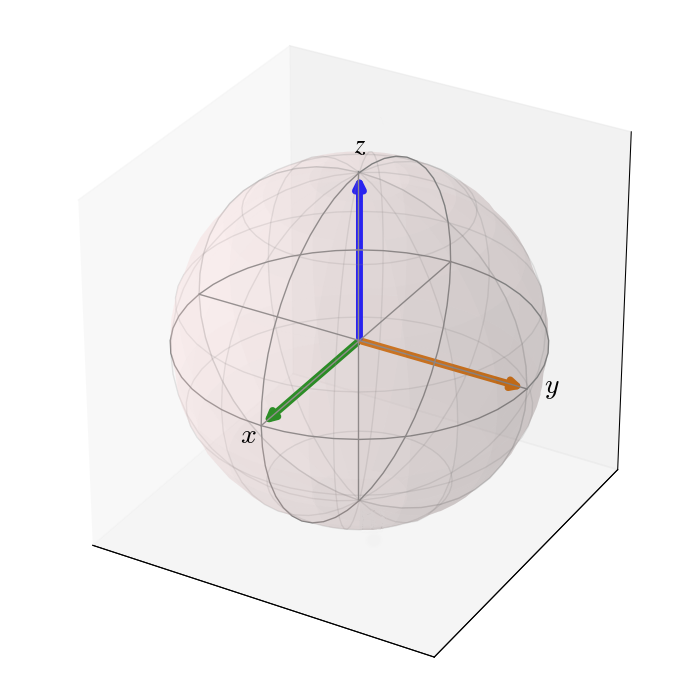
\includegraphics[scale=0.3]{sphere.png}
% 	\end{minipage}
% 	\begin{minipage}{0.55\linewidth}
% 	\begin{itemize}
% 			\item There are three coordinate functions on
%                           the sphere: $x$, $y$ and $z$.
% 	\item The Toeplitz quantizations of these three functions are
%           the spin operators, with $S=\frac{N}{2}$.
% 	\end{itemize}\end{minipage}
% \end{frame}

% \section{The smallest eigenvalue}
% \begin{frame}\frametitle{A priori localization}
% 	\begin{itemize}
% 		\item In the classical model, in order to minimize the
%                   energy, one picks any point where the energy is minimal.
% 		\item What happens for an eigenvector associated with
%                   the smallest eigenvalue of $T_N(h)$, as $N\to +\infty$ ?
% 	\end{itemize}
% 	\only<1>{\begin{prop}[Charles 00]
% 		An eigenvector with minimal eigenvalue is
%                 uniformly $O(N^{-\infty})$ outside any fixed
%                 neighbourhood of $\{h=min(h)\}$.
% 	\end{prop}
% Can we get a more precise result?}
% 	\only<2>{\begin{prop}[D. 16]
%             If the minimal set is non-degenerate, then for every
%             $\delta\in [0,1/2)$, an eigenvector with minimal
%             eigenvalue is uniformly $O(N^{-\infty})$ outside a
%             neighbourhood of $\{h=min(h)\}$ with size $N^{-\delta}$.
% 	\end{prop}}

% \end{frame}

% \begin{frame}
%   \frametitle{Proof for localization speed}
%   Let $(u_N)$ be a sequence of unit eigenfunctions with minimal
%   energy $(\lambda_N)$. Assume $\min(h)=0$.

%   We prove by induction on $k$ that $$\langle u_n,h^ku_n\rangle =
%   O(N^{-k}).$$\vspace{-2em}
%   \begin{itemize}
%   \uncover<2->{\item Hard part: $k=1$ (test $T_N(h)$ against a coherent state centred on
%   a minimal point).}

%   \uncover<3>{\item Easy part: induction. $$\langle u_n,h\star h u_n\rangle =
%   \lambda_N^2 + O(N^{-\infty}),$$ where $h\star h = h^2+N^{-1}c_1(h,h)+ O(N^{-2})$.

%   Now $c_1(h,h)\leq Ch$.}\end{itemize}
% \end{frame}
% \subsection{Wells}
% \begin{frame}
%   \frametitle{Case of several wells}
%   \begin{minipage}[l]{0.3\linewidth}
%     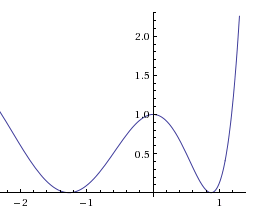
\includegraphics[width=\linewidth]{wells.png}
%   \end{minipage}
%   \begin{minipage}[r]{0.65\linewidth}
%     What can be said if $h$ is minimal on non-degenerate critical
%     points?
    
%     \uncover<2->{
%       \begin{thm}[D. 16]
%         The eigenvectors of minimal eigenvalue concentrate only on
%         ``minimal'' points. Eigenvectors and eigenvalue have an
%         asymptotical expansion.
%       \end{thm}
%     }

%     \uncover<3>{What is minimized ? The $\mu_1$ of the hessian at this
%       point.}
%   \end{minipage}
% \end{frame}

% \begin{frame}
%   \frametitle{Case of wells: idea of proof}
%   \begin{itemize}
%   \item By making more precise the previous argument, we have a lower
%     bound for the first eigenvalue.
%   \item The upper bound and a spectral gap are obtained by
%     $N^{-K}$-quasimode for fixed $K$.
%   \end{itemize}

% We remark that the quasimodes are exponentially localized, but this
% does not imply that the true eigenfunction is also localized.
% \end{frame}

% \subsection{Miniwells}

% \begin{frame}
%   \frametitle{Case of submanifold wells}
%   \begin{itemize}
% \item What can be said if $h$ is minimal on a submanifold, with
%   non-degenerate transverse hessian?
%   \item $\Rightarrow$ Same conclusion. (D.)\end{itemize}
%    \begin{minipage}[l]{0.3\linewidth}
% 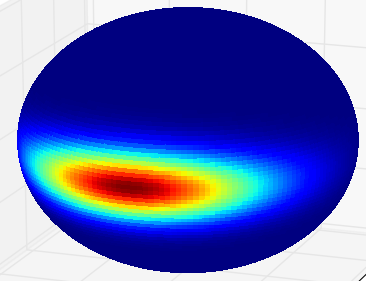
\includegraphics[scale=0.3]{35.png}\end{minipage}\begin{minipage}[r]{0.65\linewidth}
% As $N$ grows, the state concentrates on the miniwell and is more
% and more squeezed.\end{minipage}
% \end{frame}
% \begin{frame}
% \frametitle{Miniwells in physics}
%     It really happens in physics ! For instance, with
%       antiferromagnetic spins on a triangle graph.
% \begin{minipage}[l]{0.3\linewidth}
%       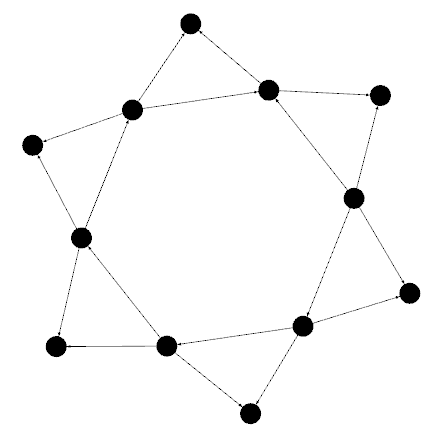
\includegraphics[scale=0.2]{hexa.png}\end{minipage}\begin{minipage}[r]{0.65\linewidth}
%       It is conjectured that the minimal configurations are planar, in
%       some cases.
%       \end{minipage}

% \end{frame}
% \subsection{Conjectures}
% \begin{frame}
%   \frametitle{Conjectures}
%   \begin{description}
%   \item[Exponential Localization] For now we only have
%     $O(N^{-\infty})$ estimates for localisation. Can we hope for
%     $O(\exp(-cN))$ estimates ?
%   \item[Thermodynamical limit] Instead of considering a fixed manifold
%     $M$, we look at a particular symbol on $M^n$, and we let $n\to
%     +\infty$. What is the behaviour vis-à-vis the semiclassical limit?
%   \end{description}

% These two questions should be linked with each other.
% \end{frame}
\end{document}
%%% Local Variables:
%%% mode: latex
%%% TeX-master: t
%%% End:
